\section{Aufgaben}
\subsection{Workflow}
\begin{frame}{Workflow}
 \begin{itemize}
  \item \target {\em default} Konfiguration
  \begin{itemize}
   \item herstellen
   \item auf SD-Karte
   \item ausprobieren
  \end{itemize}
  \item Die {\em default} Konfiguration ändern:
  \begin{itemize}
   \item Internet über USB:
   
\begin{minipage}{0.75\linewidth}
\dirtree{%
.1 Device Drivers.
.2 USB support.
.3 USB Gadget Support.
.4 USB Gadget Drivers.
}
\end{minipage}
   \item nur eine CPU
   \item keine ALSA Soundkarte
   \item ... 
  \end{itemize}
%  \item füge Treiber für WLAN hinzu
 \end{itemize}
\end{frame}

\begin{frame}{USB-Gadget}

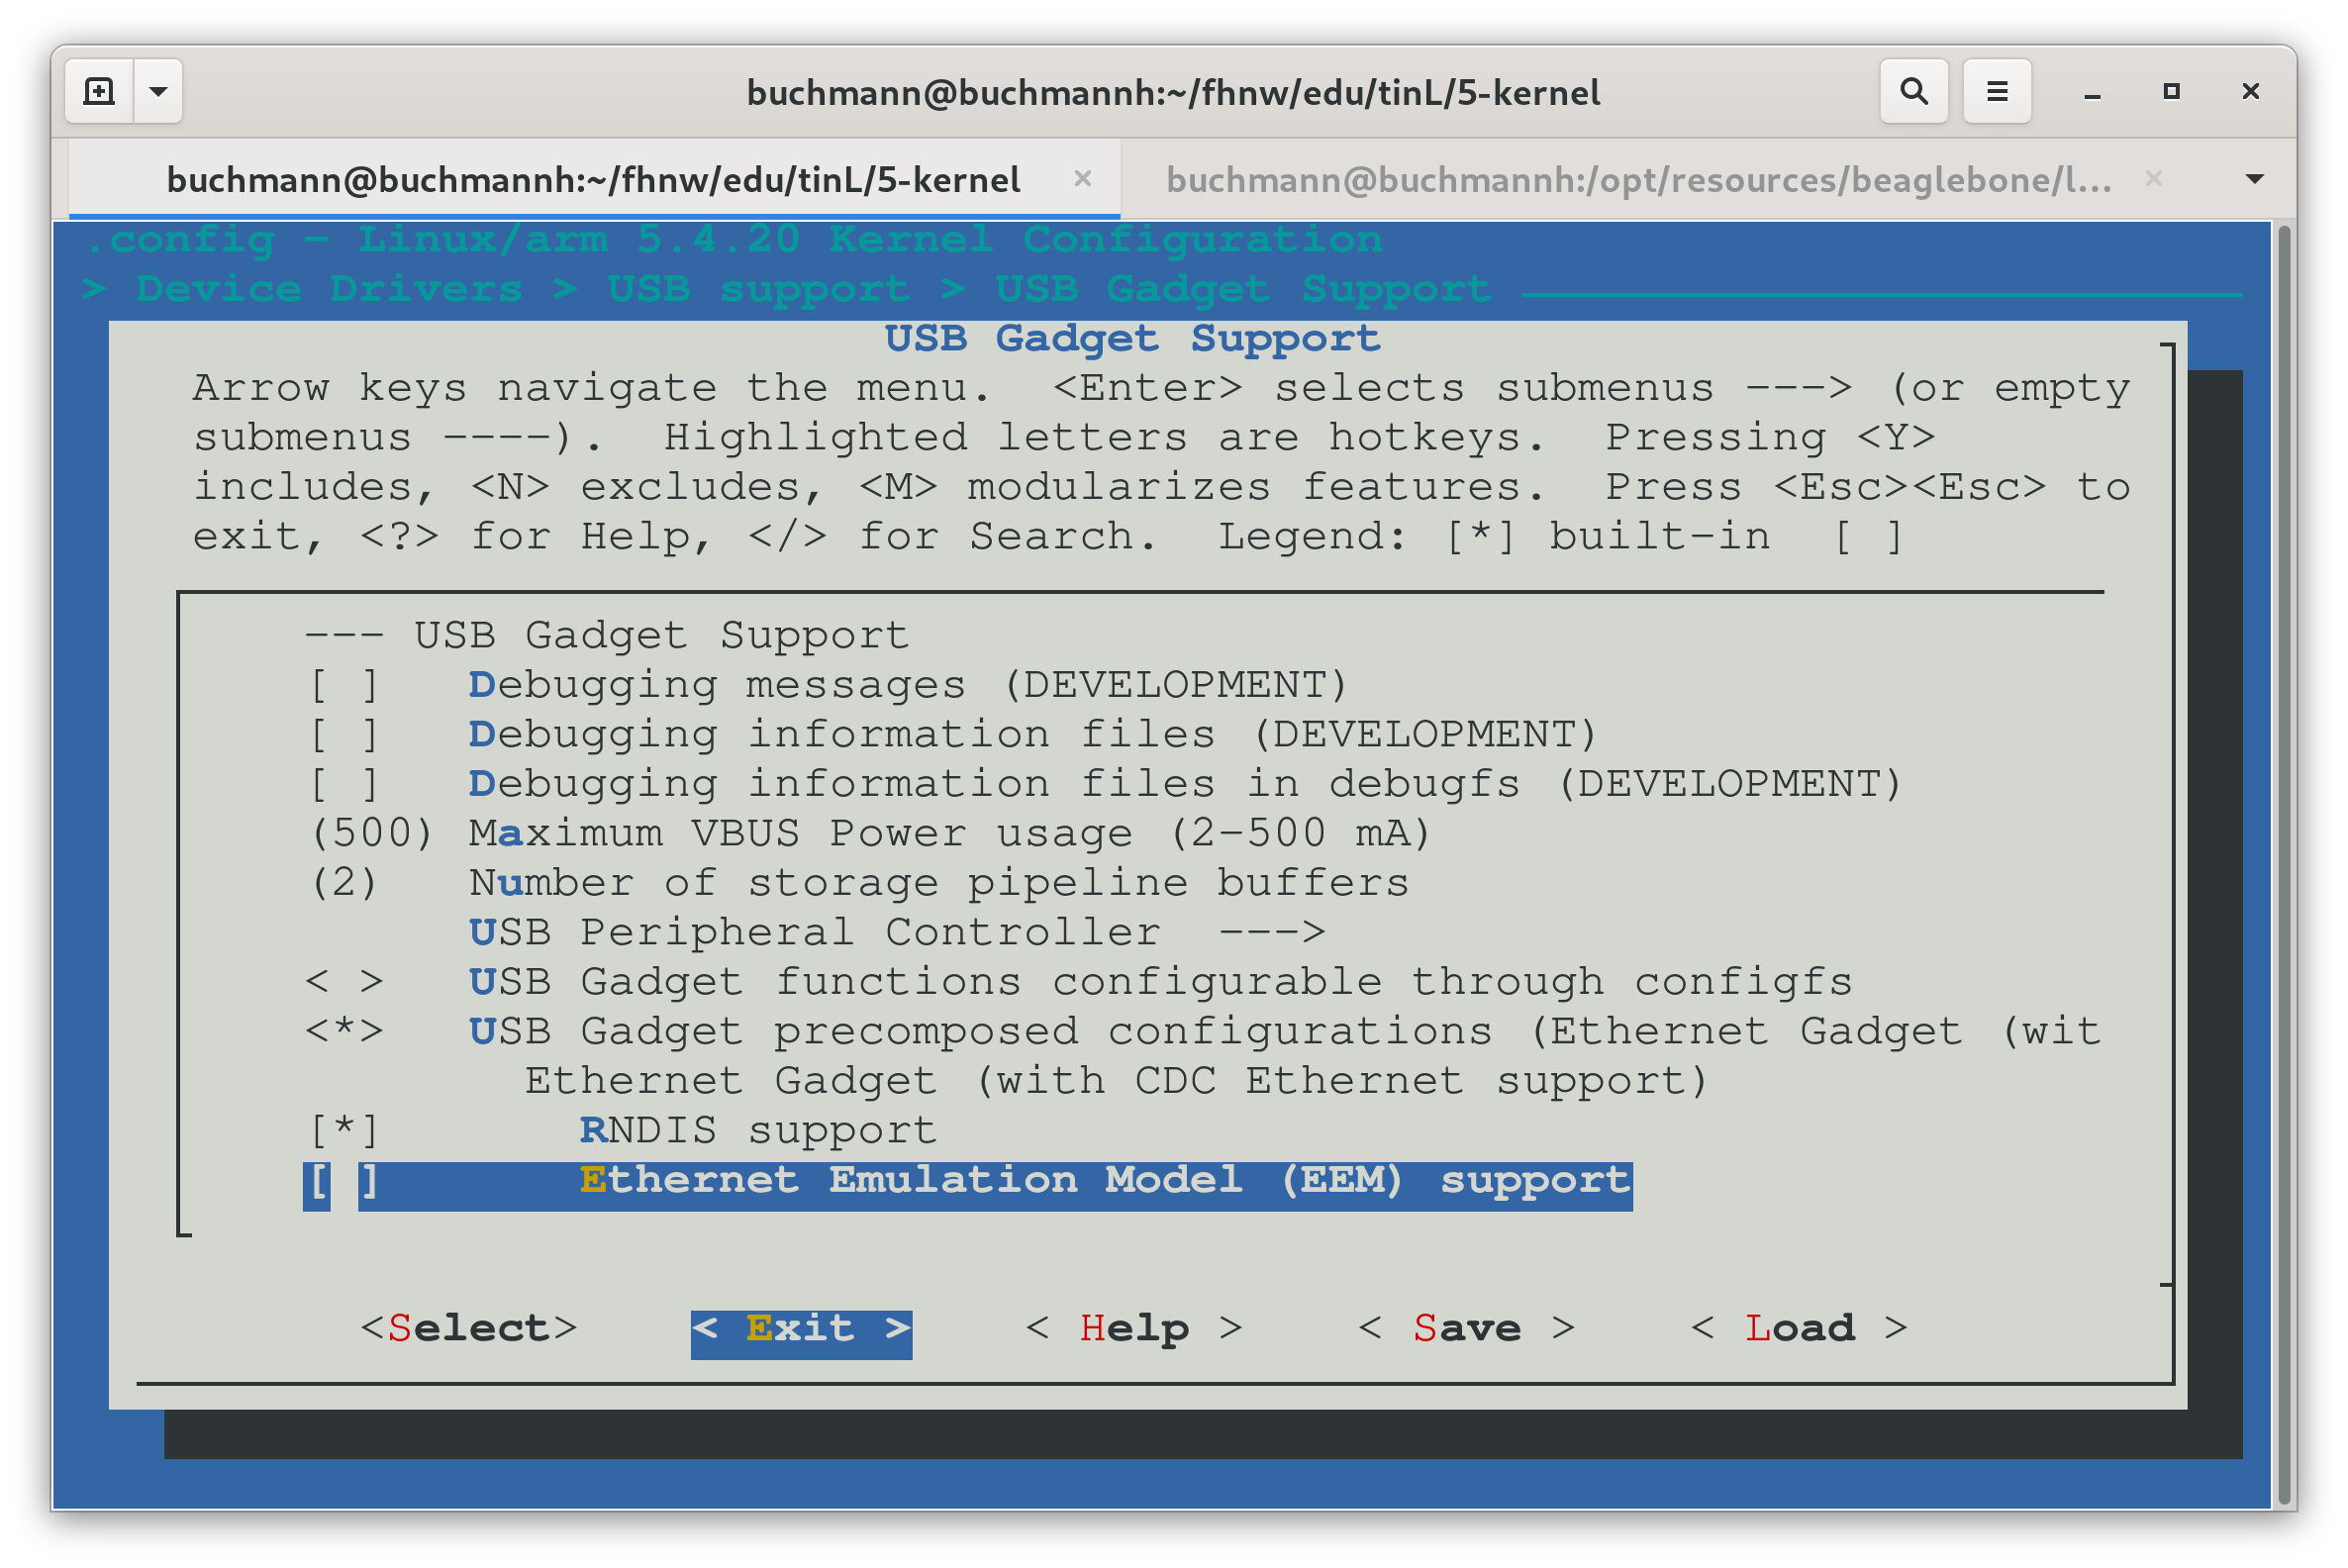
\includegraphics[width=1\textwidth]{usb-gadget.png}
\end{frame}

\begin{frame}{Die beteiligten Files}
 \begin{itemize}
  \item \cod{zImage} der {\em kernel}
  \item \cod{am335x-boneblack-wireless.dtb} der {\em device tree}
 \end{itemize}
\end{frame}
